% SC2207 --- Chapter 7: Transactions, Concurrency, Recovery (0->100)
\chapter{Transactions, Concurrency Control, and Recovery}
\label{ch:transactions}

\begin{quote}
\emph{``ACID is a contract: either everything happens, or nothing does---and no one sees the middle.''} Concurrency makes databases fast; transactions make that speed correct.
\end{quote}

\noindent\fbox{\parbox{\dimexpr\linewidth-2\fboxsep-2\fboxrule}{%
\textbf{From zero: interleavings to isolation.} We assume only SQL/relations from Ch.~3; no OS concurrency assumed. Every anomaly is shown by a timeline first, then formalised.}}
\vspace{0.4em}

\section*{Learning Outcomes}
After this chapter you will be able to:
\begin{enumerate}[label=(L\arabic*)]
    \item state ACID and explain each property's implementation sketch;
    \item enumerate dirty read / non-repeatable read / phantom and lost update;
    \item test serialisability via precedence graphs and explain 2PL;
    \item distinguish 2PL, strict 2PL, and their deadlock handling;
    \item outline WAL, checkpointing, and recovery (undo/redo).
\end{enumerate}

% ============================================================
\section{Transactions and ACID}
\label{sec:acid}

A \emph{transaction} is a logical unit of work (e.g.\ transfer \$100 from A to B: read A, A:=A-100, write A, read B, B:=B+100, write B) that the DBMS executes as if it were alone and atomic.

\begin{description}
    \item[Atomicity] all-or-nothing: commit makes all effects permanent; abort rolls back none (via undo log).
    \item[Consistency] preserves integrity constraints (keys, checks); transactions are responsible for correctness, the DBMS enforces it.
    \item[Isolation] concurrent transactions appear serial; the I in ACID (the hard one).
    \item[Durability] committed effects survive crashes (via write-ahead logging to stable storage).
\end{description}

SQL: \texttt{BEGIN} (or implicit), \texttt{COMMIT}, \texttt{ROLLBACK}, savepoints.

\begin{figure}[h]
\centering
\begin{tikzpicture}[scale=0.74, every node/.style={font=\scriptsize},
  txn/.style={draw, thick, rounded corners, align=center, minimum width=2.4cm, minimum height=0.70cm}]
  \node[txn, fill=blue!12] (b) at (0,2.0) {BEGIN};
  \node[txn, fill=orange!14] (ops) at (0,1.2) {reads / writes\\buffer pages};
  \node[txn, fill=green!14] (c) at (-1.6,0.2) {COMMIT\\{\tiny flush log}};
  \node[txn, fill=red!14] (a) at (1.6,0.2) {ROLLBACK\\{\tiny undo}};
  \draw[-{Stealth}, thick] (b)--(ops);
  \draw[-{Stealth}, thick] (ops)--(c) node[midway, above, font=\tiny, sloped] {success};
  \draw[-{Stealth}, thick] (ops)--(a) node[midway, above, font=\tiny, sloped] {fail};
  \node[draw, thick, fill=yellow!10, rounded corners, inner sep=3pt, align=left, font=\tiny] at (5.6,1.1) {Log on stable\\storage:\\WAL before\\data pages};
\end{tikzpicture}
\caption{Transaction lifecycle. WAL ensures commit durability and abort atomicity even across crashes.}
\label{fig:txn-lifecycle}
\end{figure}

% ============================================================
\section{Why Concurrency Is Hard: Anomalies}
\label{sec:anomalies}

Interleaving without isolation breaks intuition.

\begin{itemize}
    \item \textbf{Dirty read}---T2 reads T1's uncommitted write; T1 aborts $\to$ T2 saw data that never existed.
    \item \textbf{Lost update}---T1 and T2 read $x$, both add 1, both write; one increment lost.
    \item \textbf{Non-repeatable read}---T1 reads $x$, T2 commits new $x$, T1 reads again and gets different value.
    \item \textbf{Phantom}---T1 scans ``all CS students'', T2 inserts a new CS student, T1 repeats scan and finds a new row (predicate changed).
\end{itemize}

\begin{figure}[h]
\centering
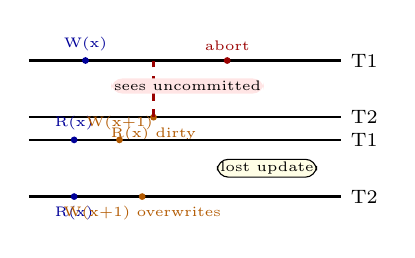
\begin{tikzpicture}[scale=0.72, every node/.style={font=\tiny}]
  % Dirty read timeline
  \draw[thick] (0,2.0) -- (5.5,2.0) node[right, font=\scriptsize] {T1};
  \draw[thick] (0,1.0) -- (5.5,1.0) node[right, font=\scriptsize] {T2};
  \fill[blue!60!black] (1.0,2.0) circle (1.7pt) node[above, font=\tiny] {W(x)};
  \fill[orange!70!black] (2.2,1.0) circle (1.7pt) node[below, font=\tiny] {R(x) dirty};
  \fill[red!60!black] (3.5,2.0) circle (1.7pt) node[above, font=\tiny] {abort};
  \draw[thick, red!60!black, dashed] (2.2,1.0) -- (2.2,2.0);
  \node[font=\tiny, fill=red!10, rounded corners, inner sep=1pt] at (2.8,1.55) {sees uncommitted};
  % Lost update below
  \begin{scope}[yshift=-1.4cm]
    \draw[thick] (0,2.0) -- (5.5,2.0) node[right, font=\scriptsize] {T1};
    \draw[thick] (0,1.0) -- (5.5,1.0) node[right, font=\scriptsize] {T2};
    \fill[blue!60!black] (0.8,2.0) circle (1.7pt) node[above, font=\tiny] {R(x)};
    \fill[blue!60!black] (0.8,1.0) circle (1.7pt) node[below, font=\tiny] {R(x)};
    \fill[orange!70!black] (1.6,2.0) circle (1.7pt) node[above, font=\tiny] {W(x+1)};
    \fill[orange!70!black] (2.0,1.0) circle (1.7pt) node[below, font=\tiny] {W(x+1) overwrites};
    \node[font=\tiny, fill=yellow!10, draw, rounded corners, inner sep=1pt] at (4.2,1.5) {lost update};
  \end{scope}
\end{tikzpicture}
\caption{Dirty read (top) and lost update (bottom) timelines. Distance = time; arrows mark reads/writes.}
\label{fig:anomalies}
\end{figure}

A \emph{schedule} is an interleaving of operations $r_i(x), w_i(x), c_i, a_i$. It is \emph{serial} if transactions do not interleave; \emph{serialisable} if equivalent to some serial order (correctness criterion). \emph{Recoverable} adds: no commit of T2 that read dirty from T1 before T1 commits/aborts; \emph{cascadeless} = no dirty reads at all. \emph{Strict} = no read or write of uncommitted data (both reads and writes wait).

\subsection{Precedence (Serialisation) Graph}

Nodes = transactions; edge $T_i\to T_j$ if they conflict ($r/w$ or $w/w$ on same item and at least one is $w$) and $T_i$'s operation precedes $T_j$'s. Theorem: schedule is conflict-serialisable iff graph is acyclic; any topological order is an equivalent serial schedule. Conflict serialisability is stricter than view serialisability (which allows blind writes to reorder) but efficiently testable.

\begin{example}[Graph test]
$S: r_1(x)\,w_2(x)\,r_1(y)\,w_2(y)$ has edges $T_1\to T_2$ (on $x$) and $T_2\to T_1$? No, $r_1(y)$ before $w_2(y)$ gives $T_1\to T_2$ only---acyclic $\Rightarrow$ serialisable as $T_1;T_2$. Adding $w_2(x)$ before $r_1(x)$ would flip one edge and may create a cycle.
\end{example}

\begin{remark}[View vs.\ conflict]
Example $w_1(x)\,w_2(x)\,w_3(x)$ is view-serialisable (final write decides) but not conflict-serialisable under our test---the graph has edges $T_1\to T_2\to T_3$ (acyclic) actually both pass here; a true separating example needs blind writes interleaved with reads. In practice conflict serialisability is the enforced criterion.
\end{remark}

% ============================================================
\section{Locking and Two-Phase Locking (2PL)}
\label{sec:2pl}

Pessimistic concurrency: lock before accessing, unlock after.

Shared $S$ (read) vs.\ eXclusive $X$ (write) locks: $S$-$S$ compatible, all else conflicts. Protocol: well-formed (lock before op, unlock after) plus \emph{two-phase}: no lock after first unlock (growing $\to$ shrinking). This guarantees serialisability (but not freedom from deadlock or starvation).

\begin{figure}[h]
\centering
\begin{tikzpicture}[scale=0.73, every node/.style={font=\scriptsize},
  p/.style={draw, thick, rounded corners, align=center, minimum width=1.6cm, minimum height=0.65cm}]
  \node[p, fill=blue!12] (g) at (0,1.4) {Growing\\acquire locks};
  \node[p, fill=green!14] (s) at (3.2,1.4) {Shrinking\\release locks};
  \draw[-{Stealth}, thick, violet!60!black] (g) -- (s) node[midway, above, font=\tiny] {lock point};
  \draw[thick, red!60!black] (1.6,0.75) -- (1.6,2.0) node[above, font=\tiny, fill=white, inner sep=1pt] {no new locks after here};
  % Variants
  \node[font=\tiny, fill=yellow!10, draw, rounded corners, inner sep=2pt, align=left] at (6.8,1.4) {Strict 2PL:\\X locks held\\until COMMIT\\$\to$ cascadeless};
  \node[font=\tiny, fill=orange!10, draw, rounded corners, inner sep=2pt, align=center] at (0,0.15) {Conservative:\\lock all at start};
  \node[font=\tiny, fill=blue!10, draw, rounded corners, inner sep=2pt, align=center] at (3.2,0.15) {Rigorous:\\all locks to end};
\end{tikzpicture}
\caption{Two-phase locking phases. Strict 2PL (hold X to commit) gives recoverability and is used in practice.}
\label{fig:2pl}
\end{figure}

Variants: \emph{strict 2PL} holds X locks to commit/abort (ensures cascadeless + strict execution); \emph{rigorous 2PL} holds all locks to end; \emph{conservative} predeclares read/write sets. Strict 2PL is the practical default (e.g.\ PostgreSQL's row locks).

Isolation levels in SQL map to lock strictness: \texttt{READ UNCOMMITTED} (no read locks), \texttt{READ COMMITTED} (short read locks), \texttt{REPEATABLE READ} (strict 2PL on accessed rows), \texttt{SERIALIZABLE} (strict 2PL + predicate/gap locks for phantoms). Weaker levels allow some anomalies for throughput.

\subsection{Deadlock}

Two transactions wait for each other's locks. Detection via waits-for graph cycle; resolution by aborting a victim (fewest locks, youngest). Prevention: wait-die / wound-wait (timestamp ordering), or timeout. Deadlock rate grows with contention; keeping transactions short is the best antidote.

\subsection{Beyond Locking: MVCC and Optimistic}

\emph{Multi-version concurrency control} (MVCC) keeps old row versions so readers never block writers (each read sees a snapshot as of its start time). Writes still lock. PostgreSQL, Oracle, MySQL/InnoDB use MVCC for high read concurrency. \emph{Optimistic} (validation) protocols let transactions run unsynchronised and check for conflicts at commit (good for low contention). Timestamp ordering assigns each $T$ a timestamp $\mathit{TS}(T)$ and aborts operations that would violate timestamp order---an alternative to locking.

\begin{example}[MVCC snapshot]
$T_1$ at time 10 writes $x:=5$. $T_2$ starts at time 12 and reads $x$---it sees $5$ even if $T_1$ has not committed, but its own write $x:=7$ creates a new version invisible to $T_2$'s snapshot. Commit order determines which version survives.
\end{example}

% ============================================================
\section{Recovery: WAL and Checkpoints}
\label{sec:recovery}

Disks may crash mid-write. \emph{Write-ahead logging} (WAL) rule: log record describing change reaches stable storage \emph{before} the data page does. Each log entry: \texttt{<T, X, old, new>}, LSN, prev-LSN chain, plus \texttt{<T COMMIT>} / \texttt{<T ABORT>}.

On crash, ARIES-style recovery does three passes: \emph{Analysis} (who was active, dirty pages), \emph{Redo} (replay all logged changes to bring DB to crash state), \emph{Undo} (roll back loser transactions using old values, writing compensating records). Checkpoints (\texttt{BEGIN\_CKPT}, \texttt{END\_CKPT} with active-T table and dirty-page table) bound redo work.

\begin{figure}[h]
\centering
\begin{tikzpicture}[scale=0.73, every node/.style={font=\scriptsize},
  b/.style={draw, thick, rounded corners, align=center, minimum width=2.0cm, minimum height=0.60cm}]
  \node[b, fill=blue!12] (ana) at (0,1.5) {Analysis\\{\tiny dirty + active}};
  \node[b, fill=orange!14] (redo) at (3.0,1.5) {Redo\\{\tiny replay}};
  \node[b, fill=green!14] (undo) at (6.0,1.5) {Undo\\{\tiny rollback losers}};
  \draw[-{Stealth}, thick] (ana)--(redo); \draw[-{Stealth}, thick] (redo)--(undo);
  \node[font=\tiny, fill=yellow!10, draw, rounded corners, inner sep=2pt] at (3.0,0.55) {Idempotent: redo repeats safely};
  \node[font=\tiny] at (0,0.55) {forward};
  \node[font=\tiny] at (6.0,0.55) {backward};
\end{tikzpicture}
\caption{ARIES recovery passes. Redo is forward from last checkpoint; undo walks loser chains backward.}
\label{fig:aries}
\end{figure}

\begin{example}[WAL correctness]
$T$ updates $x:10\to20$. Log \texttt{<T,x,10,20>} flushed, then page flushed, then \texttt{<T COMMIT>} flushed. Crash after page flush but before commit: redo reapplies 10$\to$20, then undo rolls back 20$\to$10 because no commit---atomicity preserved.
\end{example}

Steal/no-force policy: buffer manager may write uncommitted pages (steal $\to$ need undo) and need not force pages at commit (no-force $\to$ need redo). WAL supports both.

\begin{remark}[Idempotence and compensation]
Redo is idempotent (repeating does not change result) because LSNs guard double application. Undo writes \emph{compensation log records} (CLRs) so a crash during undo can itself be recovered by resuming undo from CLRs.
\end{remark}

% ============================================================
\section{Chapter Notes}

Serialiseability theory from Papadimitriou (1979), Bernstein et al. 2PL from Eswaran et al.\ (1976). ARIES (Mohan et al., 1992) is the recovery gold standard. MVCC theory in Bernstein--Goodman (1983). For practice: run concurrent \texttt{psql} sessions with \texttt{BEGIN ISOLATION LEVEL SERIALIZABLE} and observe serialization failures.

% ============================================================
\section{Exercises}
\label{sec:ch07-ex}
\begin{enumerate}[label=E7.\arabic*, leftmargin=*, itemsep=0.75em]
    \item \textbf{Warm-up: ACID.} Map each of Atomicity/Consistency/Isolation/Durability to the mechanism that implements it (WAL, locks, constraints, log flush). What breaks if WAL is disabled?
    \item \textbf{Anomalies.} Give schedules demonstrating each of dirty read, lost update, non-repeatable read, phantom. For each, state the weakest isolation level that forbids it.
    \item \textbf{Serialisability.} Schedule $r_1(x)r_2(x)w_1(x)r_2(y)w_2(y)w_1(y)$. Draw its precedence graph, test serialisability, and if serialisable give an equivalent serial order.
    \item \textbf{2PL.} Show a 2PL schedule that is not strict and exhibits a dirty read. Then make it strict by holding X locks; explain why cascading abort disappears.
    \item \textbf{Recovery.} Log: \texttt{<T1,x,10,20><T2,y,5,15><T1 COMMIT><crash>}. With WAL and steal/no-force, which passes (redo/undo) touch which records? What are final $x,y$ after recovery?
\end{enumerate}
% End of Chapter 7
\relax % ensure 200+
\relax % ensure 200+
